\documentclass[a4paper, 12pt]{article}

%-----------------------------------------------------
%                      PACKAGES
% ----------------------------------------------------
\usepackage[T1]{fontenc}
\usepackage[latin9]{inputenc}
\usepackage{fancyhdr}
\usepackage{geometry}
\usepackage[colorlinks=true, linkcolor=blue,citecolor=blue, urlcolor=blue]{hyperref}
\usepackage{indentfirst}
\usepackage{graphicx}
\usepackage{float}
\usepackage{setspace}
\usepackage{amsmath}
\usepackage{amssymb}
\usepackage{multirow}
\usepackage[table,xcdraw]{xcolor}
\usepackage{colortbl}
\usepackage{tabularx,booktabs}
\usepackage{enumerate}
\usepackage{titlesec}
\usepackage{caption}
\usepackage{subcaption}
\usepackage{nicefrac, xfrac}
\usepackage{subfiles}
\usepackage{mathtools}
\usepackage{bm}
\usepackage{tikz}
\usepackage[mode=buildnew]{standalone}
\usepackage{systeme}
\usepackage{stmaryrd}
\usepackage{import}
\usepackage[brazil]{babel} 
\usepackage{times}
\usepackage{pgfplots}
\usepackage{makecell}
\usepackage{threeparttable}
\usepackage{ragged2e}
\usepackage{tocloft}
\usepackage{booktabs}
\usepackage[acronym]{glossaries}
\usepackage{pdfpages}
\usepackage{lipsum}
\usepackage{hyphenat} 
\usepackage{xspace}
\usepackage{abntex2cite}

%-----------------------------------------------------
%               DOCUMENT SETTINGS
% ----------------------------------------------------
\geometry{a4paper,top=30mm,bottom=20mm,left=30mm,right=20mm}

\pgfplotsset{compat=1.17} 

\numberwithin{equation}{section}
\counterwithin{figure}{section}

% Defining spaces between lines
\setstretch{1.5} 

\graphicspath{{Figures/}}

\tikzset{
	font={\fontsize{11pt}{12}\selectfont}}

\setcounter{secnumdepth}{4}
\setcounter{tocdepth}{4}

% defining the height of table cells
\renewcommand{\arraystretch}{1.5}

% defining the gradient, divergence and curl operators
\newcommand{\grad}[1]{\nabla #1}
\renewcommand{\div}[1]{\nabla \cdot #1}
\newcommand{\curl}[1]{\nabla \times #1}

\def\textcite#1{\citeauthoronline{#1} \cite{#1}}
%-----------------------------------------------------
%              PRE TEXTUAL ELEMENTS
% ----------------------------------------------------
\newenvironment{epigrafe}{\newpage\mbox{}\vfill\hfill\begin{minipage}[t]{0.5\textwidth}}
{\end{minipage}\newpage}

%-----------------------------------------------------
%                     DOCUMENT 
% ----------------------------------------------------
\begin{document}
% ------- WORK INFORMATION -------
\author{Carlos Henrique Chama Puga}
\newcommand{\RA}{195416}

\title{Lista 1 \\ Derivadas, Gradiente, Divergente e Rotacional}

\newcommand{\Uni}{{Universidade Estadual de Campinas}}
\newcommand{\Fac}{{Faculdade de Engenharia Civil, Arquitetura e Urbanismo}}

\newcommand{\advisor}{Porf. Dr. Philippe Devloo}
\newcommand{\coadvisor}{Dr. Giovane Avancini}

\newcommand*{\workyear}{2024}

\makeatletter

% ------- PRE TEXTUAL PAGES -------
% Could not find another way to remove the page number from the first pages
\fancypagestyle{plain}{
    \fancyhf{}% Limpa todos os campos
    \fancyfoot[C]{}%
    \renewcommand{\headrulewidth}{0pt}%
}

\pagestyle{plain}
\def\logos{
    \noindent
    \raisebox{-.5\height}{
\includegraphics[width=2.2cm]{Figures/logo-unicamp.pdf}}

    \vspace*{1.5cm}
    
    \noindent
    \begin{center} \large
        \MakeUppercase{\Uni}\\
        \Fac\\
    \end{center}
}

\def\openningpage{
  \logos
  \vskip 35mm
  \begin{center}
    \Large
      {\bf \@title}
  \end{center}
  \vskip 25mm
  \begin{flushright}
    \large
    {\textbf{Aluno:} \\ \@author - \RA}
    \vskip 10mm
    {{\bf{Docentes}}: \\
     \advisor \\
     \coadvisor}
  \end{flushright}
    \vfill
    \large
  \begin{center}
    Campinas\\\workyear
  \end{center}
}

\openningpage % Cover page

% Table of contents
\newpage
\tableofcontents 

% from here on, the page number is shown
% Chapter first page settings
\newpage
\fancypagestyle{plain}{
    \fancyhf{}% Limpa todos os campos
    \fancyhead[R]{\thepage}%
    \renewcommand{\headrulewidth}{0pt}%
}

\fancypagestyle{headings}{%
    \fancyhf{}% Limpa todos os campos
    \fancyhead[L]{Lista 1 - Derivadas, Gradiente, Divergente e Rotacional}% Nome do trabalho à esquerda
    \fancyhead[R]{\thepage}% Numero da página à direita
    \renewcommand{\headrulewidth}{1pt}%
}

% ------- CHAPTERS -------
\pagestyle{headings}
\section{Introdu\c{c}\~{a}o} \label{sec:intro}
A primeira lista da disciplina de M\'etodos Num\'ericos compreende uma revis\~ao de c\'alculo, abordando temas como, regra da cadeia e os  operadores gradiente, divergente e rotacional. A seguir, uma breve descri\c{c}\~ao do que foi discutido em aula.

A regra da cadeia \'e uma t\'ecnica utilizada para diferenciar fun\c{c}\~oes compostas por outras fun\c{c}\~oes. O operador gradiente, quando aplicado em uma fun\c{c}\~ao escalar, gera um vetor que aponta para a dire\c{c}\~ao de maior crescimento da fun\c{c}\~ao. O operador divergente representa a densidade volum\'etrica de fluxo que sai de um campo vetorial de um volume infinitesimal em torno de um ponto. Por fim, o operador roatcional pode ser definido como a densidade de circula\c{c}\~ao de um campo vetorial em torno de um ponto, representado pelo vetor cuja dire\c{c}\~ao e magnitude denotam o eixo e a magnitude da circula\c{c}\~ao m\'axima.

A lista foi dividida em quatro exerc\'icios, cada um abordando um dos temas supracitados. A seguir, ser\~ao apresentados os exerc\'icios e suas respectivas solu\c{c}\~oes. Real\c{c}a-se que, durante toda a realiza\c{c}\~ao dos exerc\'icios, usou-se as refer\^encias \cite{stewart2007essential} e \cite{becker1981finite} para consulta.
\section{Rotacional do Gradiente de $f(x,y,z)$} \label{sec:ex1}
Seja $f(x,y,z)$ uma fun\c{c}\~ao escalar. O gradiente de $f$ \'e dado pela Eq. \eqref{eq:gradf}
\begin{equation}
    \label{eq:gradf}
    \grad{f} = \left( \frac{\partial f}{\partial x}, \frac{\partial f}{\partial y}, \frac{\partial f}{\partial z} \right).
\end{equation}

A partir de $\grad{f}$, pode-se calcular o rotacional de $\grad{f}$, dado pela Eq. \eqref{eq:rotgradf}
\begin{equation}
    \label{eq:rotgradf}
    \curl{(\grad{f})} = 
    \begin{matrix}
        \begin{vmatrix}
            \hat{i} & \hat{j} & \hat{k} \\
            \frac{\partial}{\partial x} & \frac{\partial}{\partial y} & \frac{\partial}{\partial z} \\
            \frac{\partial f}{\partial x} & \frac{\partial f}{\partial y} & \frac{\partial f}{\partial z}
        \end{vmatrix}
    \end{matrix},        
\end{equation}
em que $\hat{i}$, $\hat{j}$ e $\hat{k}$ s\~ao os vetores unit\'arios nas dire\c{c}\~oes $x$, $y$ e $z$, respectivamente.

Calculando o rotacional de $\grad{f}$, tem-se que
\begin{equation*}
    \left( \frac{\partial^2 f}{\partial y \partial z} - \frac{\partial^2 f}{\partial z \partial y} \right) \hat{i} + 
        \left( \frac{\partial^2 f}{\partial z \partial x} - \frac{\partial^2 f}{\partial x \partial z} \right) \hat{j} + 
        \left( \frac{\partial^2 f}{\partial x \partial y} - \frac{\partial^2 f}{\partial y \partial x} \right) \hat{k},
\end{equation*}
como as derivadas parciais s\~ao comutativas (Teorema de Clairaut), tem-se que
\begin{equation*}
    \curl{(\grad{f})} = \vec{0}.
\end{equation*}




\section{Divergente de Rotacional de f(x,y,z)} \label{sec:ex2}
Assumindo que a fun\c{c}\~ao ${f}(x,y,z)$ \'e um campo vetorial na forma ${f}(x,y,z) = (P, Q, R)$ e que as fun\c{c}\~oes $P(x,y,z)$, $Q(x,y,z)$ e $R(x,y,z)$ s\~ao fun\c{c}\~oes escalares, o divergente do rotacional de ${f}(x,y,z)$ \'e dado pela Eq. \eqref{eq:rot}
\begin{equation}
    \label{eq:rot}
    \nabla \times {f}(x,y,z) = \left| \begin{array}{ccc}
        \hat{i} & \hat{j} & \hat{k} \\
        \frac{\partial}{\partial x} & \frac{\partial}{\partial y} & \frac{\partial}{\partial z} \\
        P & Q & R
    \end{array} \right| = 
    \left(\begin{array}{ccc}
         \frac{\partial R}{\partial y} - \frac{\partial Q}{\partial z} \\
        \frac{\partial P}{\partial z} - \frac{\partial R}{\partial x} \\
         \frac{\partial Q}{\partial x} - \frac{\partial P}{\partial y} 
    \end{array}
    \right)
\end{equation}

O divergente de $\nabla \times {f}(x,y,z)$ \'e dado pela Eq. \eqref{eq:divrot}
\begin{equation}
    \label{eq:divrot}
    \nabla \cdot \nabla \times {f}(x,y,z) = \frac{\partial}{\partial x} \left( \frac{\partial R}{\partial y} - \frac{\partial Q}{\partial z} \right) + 
    \frac{\partial}{\partial y} \left( \frac{\partial P}{\partial z} - \frac{\partial R}{\partial x} \right) + 
    \frac{\partial}{\partial z} \left( \frac{\partial Q}{\partial x} - \frac{\partial P}{\partial y} \right).
\end{equation}

Distribuindo as derivadas parciais obt\'em-se
\begin{equation*}
    \div{(\curl{f})} = 
    \frac{\partial^2 R}{\partial x\partial y} - \frac{\partial^2 Q}{\partial x\partial z} + 
    \frac{\partial^2 P}{\partial y\partial z} - \frac{\partial^2 R}{\partial y\partial x}  + 
    \frac{\partial^2 Q}{\partial z\partial x} - \frac{\partial^2 P}{\partial z \partial y},
\end{equation*}
como pelo Teorema de Clairut, as derivadas cruzadas s\~ao iguais
\begin{equation}
    \div{(\curl{f})} = 0.
\end{equation}
\section{Regra da Cadeia em Fun\c{c}\~oes de 2 Vari\'aveis} 
Dada a fun\c{c}\~ao
\begin{equation*}
    f(x,y) = e^{x(\xi, \eta)} + e^{\sin(x(\xi, \eta) y(\xi, \eta)^3)}
\end{equation*}
calcule o gradiente relativo \`as coordenadas param\'etricas $\xi$ e $\eta$, sobre a superf\'icie parametrizada dada por:
\begin{equation*}
    \begin{cases}
        x(\xi, \eta) = \cos(\xi^2) + \sin(\eta + 1) + 5\xi \\
        y(\xi, \eta) = \sin(\xi^3) + \cos(\eta^2) + 7\eta
    \end{cases}.
\end{equation*}

\subsection{Solu\c{c}\~ao}
O exerc\'icio 3 foi feito utilizando o \textit{software} \texttt{Mathematica} e o c\'odigo utilizado pode ser encontrado no Ap\^endice \ref{sec:github}. 

O gradiente de $f$ em rela\c{c}\~ao \`as coordenadas param\'etricas $\xi$ e $\eta$ \'e dado pela regra da cadeia, expressa pela Eq. \eqref{eq:gradfxy}
\begin{equation}
    \label{eq:gradfxy}   
    \grad{f} = \begin{bmatrix}
        \frac{\partial f}{\partial \xi} \\
        \frac{\partial f}{\partial \eta}
    \end{bmatrix} = 
    \begin{bmatrix}
        \frac{\partial f}{\partial x} \frac{\partial x}{\partial \xi} + \frac{\partial f}{\partial y} \frac{\partial y}{\partial \xi} \\
        \frac{\partial f}{\partial x} \frac{\partial x}{\partial \eta} + \frac{\partial f}{\partial y} \frac{\partial y}{\partial \eta}
    \end{bmatrix}
\end{equation}
logo, basta evaluar as derivadas parciais $\frac{\partial f}{\partial x}$, $\frac{\partial f}{\partial y}$, $\frac{\partial x}{\partial \xi}$, $\frac{\partial x}{\partial \eta}$, $\frac{\partial y}{\partial \xi}$ e $\frac{\partial y}{\partial \eta}$  e depois substituir na Eq. \eqref{eq:gradfxy}.

Utilizando o \texttt{Mathematica} obt\'em-se que: 
\begin{equation*}
    \frac{\partial f}{\partial x} = e^x + y^3 e^{\sin \left(x
    y^3\right)} \cos \left(x
    y^3\right)
\end{equation*}
\begin{equation*}
    \frac{\partial f}{\partial y} = 3 y^2 e^{\sin \left(x
    y^3\right)} \cos \left(x
    y^3\right)
\end{equation*}
\begin{equation*}
    \frac{\partial x}{\partial \xi} = -2 \xi \sin \left(\xi^2\right) + 5
\end{equation*}
\begin{equation*}
    \frac{\partial x}{\partial \eta} = \cos \left(\eta + 1\right)
\end{equation*}
\begin{equation*}
    \frac{\partial y}{\partial \xi} = 3 \xi^2 \cos \left(\xi^3\right)
\end{equation*}
\begin{equation*}
    \frac{\partial y}{\partial \eta} = -2 \eta \sin \left(\eta^2\right) + 7.
\end{equation*}

Dados a complexidade e o tamanho das fun\c{c}\~oes que comp\~oem o gradiente, optou-se por apresentar um trecho do c\'odigo utilizado em que o gradiente \'e calculado. As figuras \ref{fig:dfdxi} e \ref{fig:dfdeta} mostram o c\'alculo das derivadas parciais $\frac{\partial f}{\partial \xi}$ e $\frac{\partial f}{\partial \eta}$, respectivamente.

\begin{figure}[H]
    \centering
    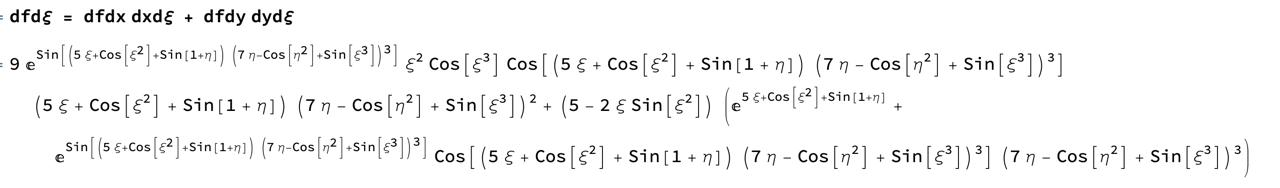
\includegraphics[scale=.38]{Figures/Ex3dfdxi.jpeg}
    \caption{C\'alculo da derivada parcial $\frac{\partial f}{\partial \xi}$.}
    \label{fig:dfdxi}
\end{figure}

\begin{figure}[H]
    \centering
    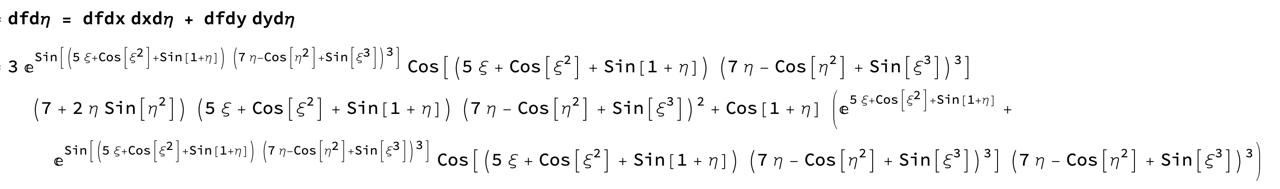
\includegraphics[scale=.38]{Figures/Ex3dfdeta.jpeg}
    \caption{C\'alculo da derivada parcial $\frac{\partial f}{\partial \eta}$.}
    \label{fig:dfdeta}
\end{figure}

Apresenta-se tamb\'em a compara\c{c}\~ao entre os resultados obtidos pela regra da cadeia programada e pelas fun\c{c}\~oes nativas do \texttt{Mathematica}

\begin{figure}[H]
    \centering
    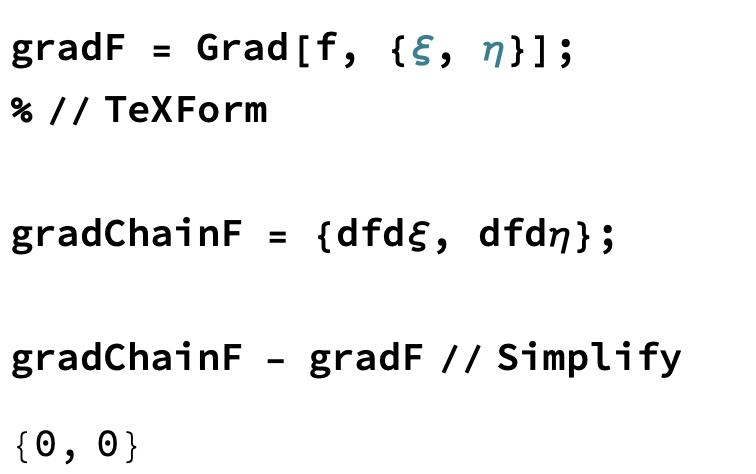
\includegraphics[scale=.22]{Figures/Ex3Comparison.jpeg}
    \caption{Compara\c{c}\~ao entre gradientes: $gradF$ - \texttt{Mathematica} e $gradChainF$ - Regra da Cadeia.}
    \label{fig:gradf}
\end{figure}

Como mostrado pela Fig. \ref{fig:gradf}, os resultados alcan\c{c}ados pela regra da cadeia e pelo \texttt{Mathematica} s\~ao iguais, j\'a que a diferen\c{c}a entre os gradientes \'e nula. Tal fato confirma que a implementa\c{c}\~ao da regra da cadeia est\'a correta. Por fim, plota-se os gr\'aficos do gradiente de $f(x(\xi, \eta), y(\xi, \eta))$ na Fig. \ref{fig:gradfplot}.

\begin{figure}[H]
    \centering
    \subfloat[\label{fig:plotGradf}]{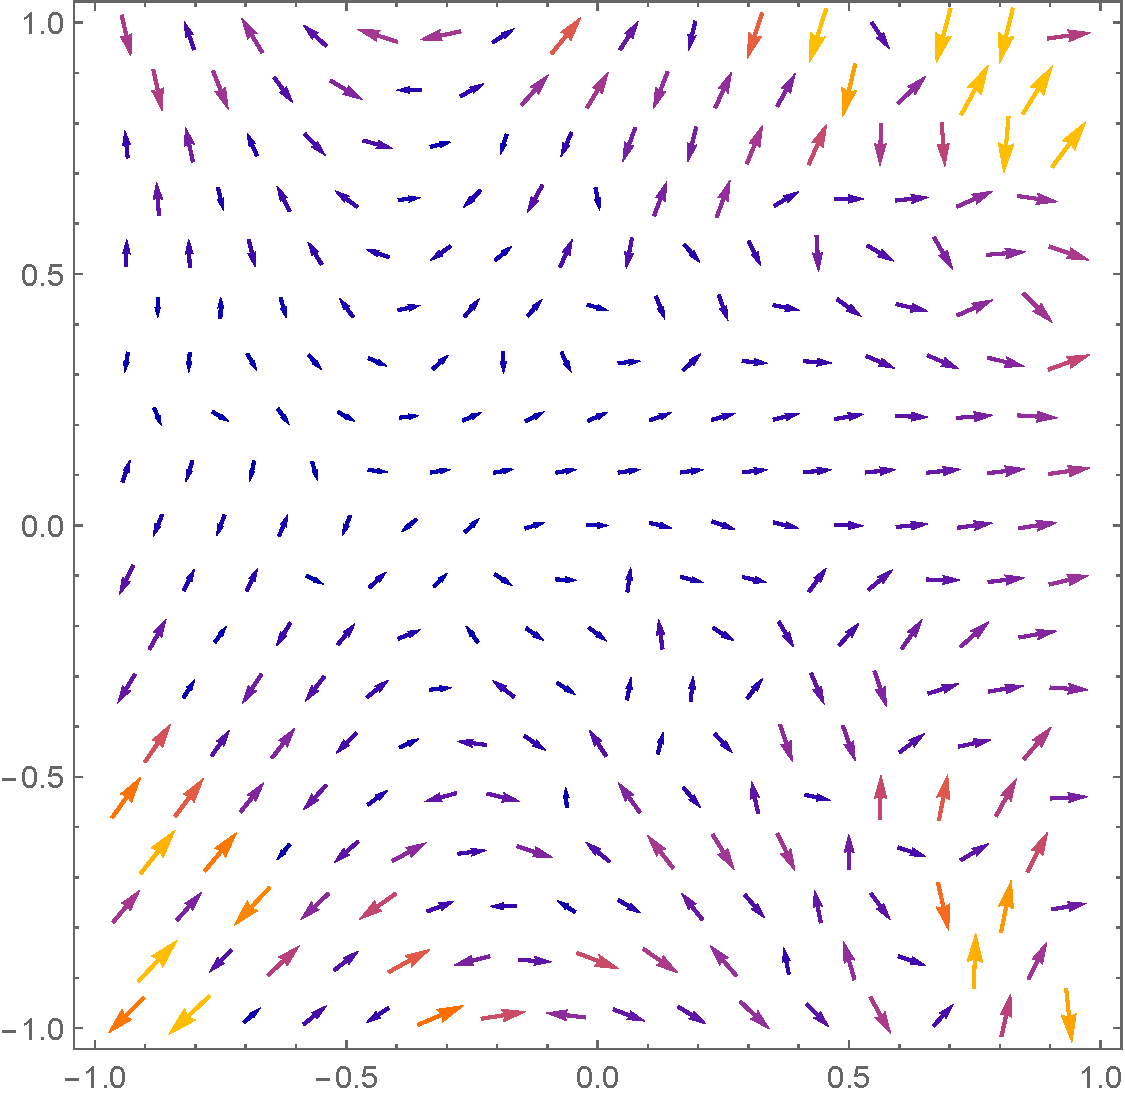
\includegraphics[width=0.49\textwidth]{Ex3GradF.pdf}}\hfill
    \subfloat[\label{fig:contourF}]{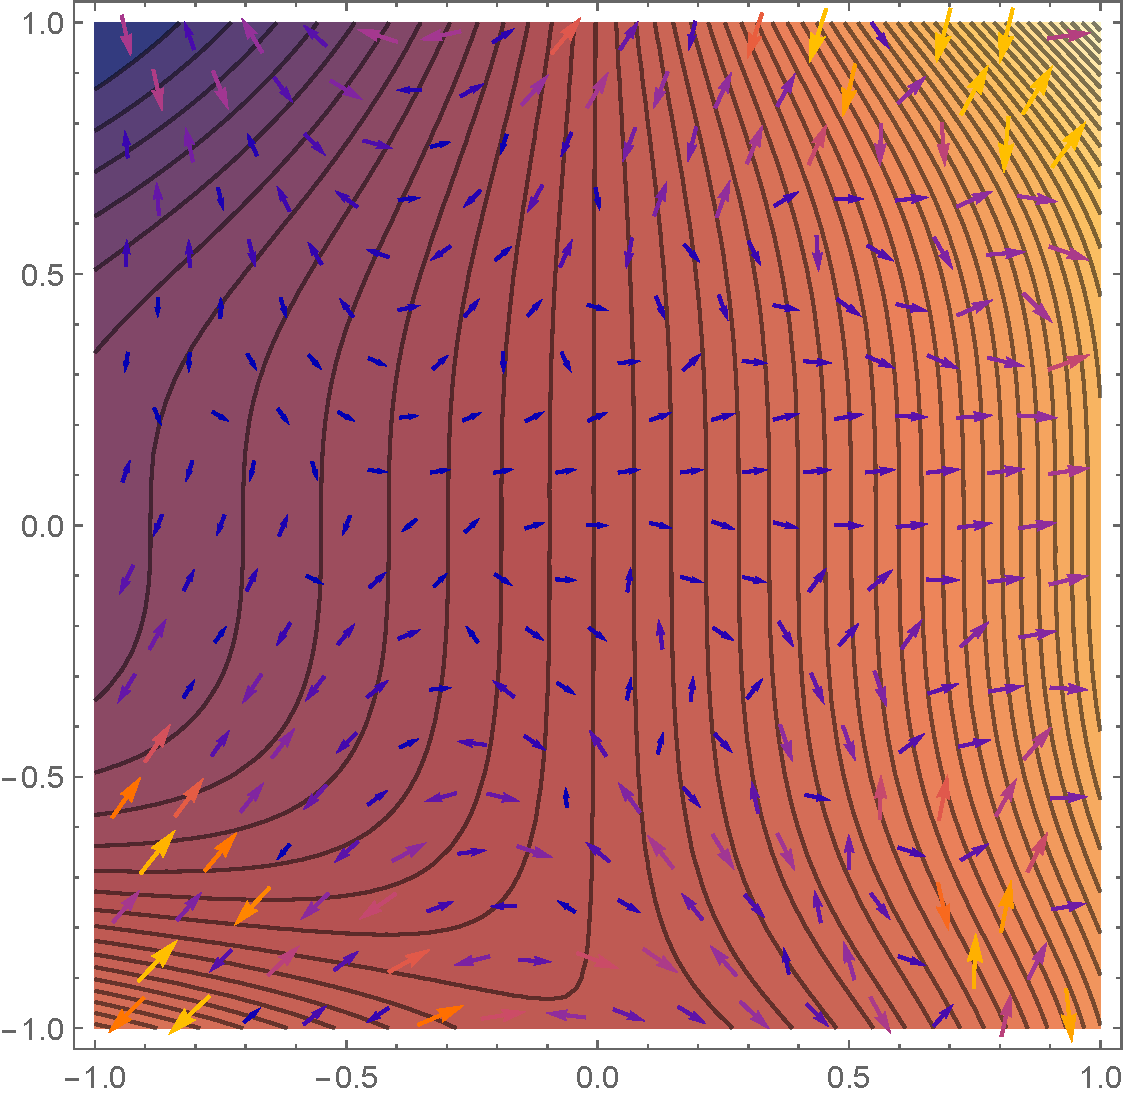
\includegraphics[width=0.49\textwidth]{Ex3ContourF.pdf}}
    \caption{Resultados: a) gradiente de $f$. b) Contorno de $f$.}
    \label{fig:gradfplot}
\end{figure}
\section{Deriva\c{c}\~oes em Fun\c{c}\~oes Mapeamento}\label{sec:derivative}
Para o exerc\'icio 4 tamb\'em foi utilizado o \textit{software} \texttt{Mathematica} para realizar os c\'alculos. A seguir a linha de pensamento base para o desenvolvimento do exerc\'icio.

Sabe-se que $x$ e $y$ s\~ao fun\c{c}\~oes diferenci\'aveis em $\xi$ e $\eta$. Com isso, os infinitesimais $d\xi$ e podem ser $d\eta$ transformado em $dx$ e $dy$ pela Eq. \eqref{eq:infinitesimal}.
\begin{equation}
    \begin{bmatrix}
        dx \\
        dy
    \end{bmatrix}
    =
    \begin{bmatrix}
        \frac{\partial x}{\partial \xi} & \frac{\partial x}{\partial \eta} \\
        \frac{\partial y}{\partial \xi} & \frac{\partial y}{\partial \eta}
    \end{bmatrix}
    \begin{bmatrix}
        d\xi\\
        d\eta
    \end{bmatrix}.
    \label{eq:infinitesimal}
\end{equation}

A matriz contendo as derivadas parciais da transforma\c{c}\~ao de coordenadas \'e chamada de matriz jacobiana ($Jac$). Invertendo o sistema de equa\c{c}\~oes \eqref{eq:infinitesimal} tem-se a Eq. \eqref{eq:inverse}, usada para encontrar as derivadas parciais de $\xi$ e $\eta$ em fun\c{c}\~ao de $x$ e $y$.
\begin{equation}
    \begin{bmatrix}
        d\xi\\
        d\eta
    \end{bmatrix}
    =
    Jac^{-1}
    \begin{bmatrix}
        dx \\
        dy
    \end{bmatrix},
    \label{eq:inverse}
\end{equation}
sendo que o inverso da Jacobiana pode ser obtido conforme Eq. \eqref{eq:inverse_jac}.
\begin{equation}
    Jac^{-1} = \frac{1}{|Jac|}
    \begin{bmatrix}
        \frac{\partial y}{\partial \eta} & -\frac{\partial x}{\partial \eta} \\
        -\frac{\partial y}{\partial \xi} & \frac{\partial x}{\partial \xi}
    \end{bmatrix},
    \label{eq:inverse_jac}
\end{equation}
com $|Jac|$ sendo o determinante da matriz jacobiana dado pela Eq. \eqref{eq:determinant}.
\begin{equation}
    |Jac| = \frac{\partial x}{\partial \xi}\frac{\partial y}{\partial \eta} - \frac{\partial x}{\partial \eta}\frac{\partial y}{\partial \xi}.
    \label{eq:determinant}
\end{equation}

Analagamente \`a Eq. \eqref{eq:infinitesimal}, pode-se escrever $d\xi$ e $d\eta$ como
\begin{equation}
    \begin{bmatrix}
        d\xi \\
        d\eta
    \end{bmatrix}
    =
    \begin{bmatrix}
        \frac{\partial \xi}{\partial x} & \frac{\partial \xi}{\partial y} \\
        \frac{\partial \eta}{\partial x} & \frac{\partial \eta}{\partial y}
    \end{bmatrix}
    \begin{bmatrix}
        dx\\
        dy
    \end{bmatrix}.
    \label{eq:infinitesimalInverse}
\end{equation}

Comparando as eqs. \eqref{eq:infinitesimal}, \eqref{eq:inverse} e \eqref{eq:inverse_jac} obt\'em-se as defini\c{c}\~oes das derivadas parciais, mostradas na Eq. \eqref{eq:finalMap}
\begin{equation}
    \label{eq:finalMap}
    \begin{cases}
        \frac{d\xi}{dx} =  \frac{1}{|Jac|}\frac{\partial y}{\partial \eta}\\
        \frac{d\eta}{dx} = -\frac{1}{|Jac|}\frac{\partial y}{\partial \xi}\\
        \frac{d\xi}{dy} = -\frac{1}{|Jac|}\frac{\partial x}{\partial \eta}\\
        \frac{d\eta}{dy} =  \frac{1}{|Jac|}\frac{\partial x}{\partial \xi}
    \end{cases}.
\end{equation}

Finalmente, pode-se aplicar a regra da cadeia para encontrar o gradiente de $f$ com rela\c{c}\~ao a $\xi$ e $\eta$ em fun\c{c}\~ao de $x$ e $y$ conforme Eq. \eqref{eq:chainRule}.
\begin{equation}
    \label{eq:chainRule}
    \grad{\hat f} = 
    \begin{bmatrix}
        \frac{\partial \hat f}{\partial x} \\
        \frac{\partial \hat f}{\partial y}
    \end{bmatrix} = 
    \begin{bmatrix}
        \frac{\partial \hat f}{\partial \xi} \frac{\partial \xi }{dx} + \frac{\partial \hat f}{\partial \eta}\frac{\partial \eta}{dx}\\
        \frac{\partial \hat f}{\partial \xi} \frac{\partial \xi }{dy} + \frac{\partial \hat f}{\partial \eta}\frac{\partial \eta}{dy}
    \end{bmatrix}
\end{equation}

A partir da Eq. \eqref{eq:chainRule} pode-se calcular o gradiente de $\hat f$ em fun\c{c}\~ao de $\xi$ e $\eta$. A seguir, os resultados obtidos pelo c\'odigo em \texttt{Mathematica}. Real\c{c}a-se que o c\'odigo na \'integra pode ser encontrado no Ap\^endice \ref{sec:github}.

Primeiramente, apresentam-se as derivadas parciais de $\hat f$ com rela\c{c}\~ao a $\xi$ e $\eta$
\begin{equation*}
    \begin{cases}
        \frac{d\hat f}{d\xi} = \frac{1}{4} (\eta -1) (-\eta -\xi -1)-\frac{1}{4} (\eta -1) (\xi -1) \\
        \frac{d\hat f}{d\eta} = \frac{1}{4} (\xi -1) (-\eta -\xi -1)-\frac{1}{4} (\eta -1) (\xi -1)  \\
    \end{cases},
\end{equation*}
as derivadas parciais de $x$ e $y$ com rela\c{c}\~ao a $\xi$ e $\eta$
\begin{equation*}
    \begin{cases}
        \frac{\partial x}{\partial \xi} = \frac{1}{4} (-2 \eta  \xi +2 \xi + 4) \\
        \frac{\partial x}{\partial \eta} = \frac{1}{4} \left(1-\xi ^2\right) \\
        \frac{\partial y}{\partial \xi} = \frac{1}{4} \left(1-\eta ^2\right) \\
        \frac{\partial y}{\partial \eta} = \frac{1}{4} (4-2 \eta  (\xi -1)) \\
    \end{cases}.
\end{equation*}
e o determinante da matriz jacobiana
\begin{equation*}
    |Jac| = \frac{1}{16} \left(\eta ^2 \left(3 \xi ^2-4 \xi +1\right)-4 \eta  \left(\xi ^2+3 \xi -2\right)+\xi ^2+8
    \xi +15\right)
\end{equation*}

Com os resultados das derivadas parciais, calcula-se o grdiente de $\hat f$. 
\begin{equation*}
    \begin{split}
        \frac{d\hat f}{dx} =&~ \frac{2 (\eta -1) (\eta  (\xi -1)-2) (\eta +2 \xi )}{\eta ^2 \left(3 \xi ^2-4 \xi +1\right)-4 \eta 
        \left(\xi ^2+3 \xi -2\right)+\xi ^2+8 \xi +15} +\\
        &+\frac{1}{16} (\xi -1) \left(\xi ^2-1\right) (2 \eta
        +\xi )
    \end{split}
\end{equation*}
\begin{equation*}
    \frac{d\hat f}{dy} = \frac{(\xi -1) \left(\eta ^2 (3 \xi -1)-\eta  (5 \xi +7)-2 \xi \right)}{\eta ^2 \left(3 \xi ^2-4 \xi
    +1\right)-4 \eta  \left(\xi ^2+3 \xi -2\right)+\xi ^2+8 \xi +15}
\end{equation*}

Por fim, apresenta-se na Fig. \ref{fig:grad4} o gr\'afico do gradiente de $\hat f$ em fun\c{c}\~ao de $x$ e $y$ e seu contorno no domínio.
\begin{figure}[H]
    \centering
    \subfloat[\label{fig:plotGradf4} Gradiente de $f$]{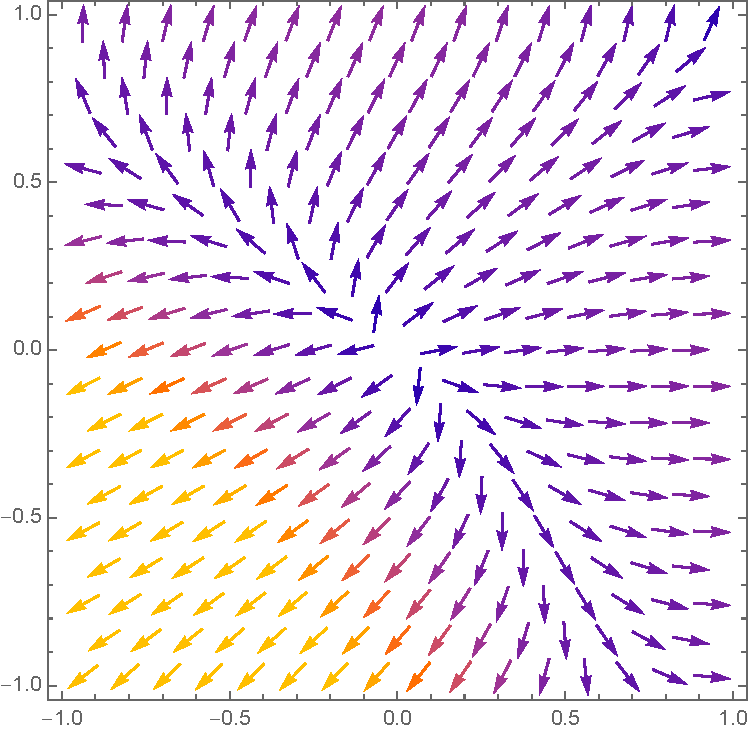
\includegraphics[width=0.49\textwidth]{Ex4GradF.pdf}}\hfill
    \subfloat[\label{fig:contourF4} Contorno de $\hat f$]{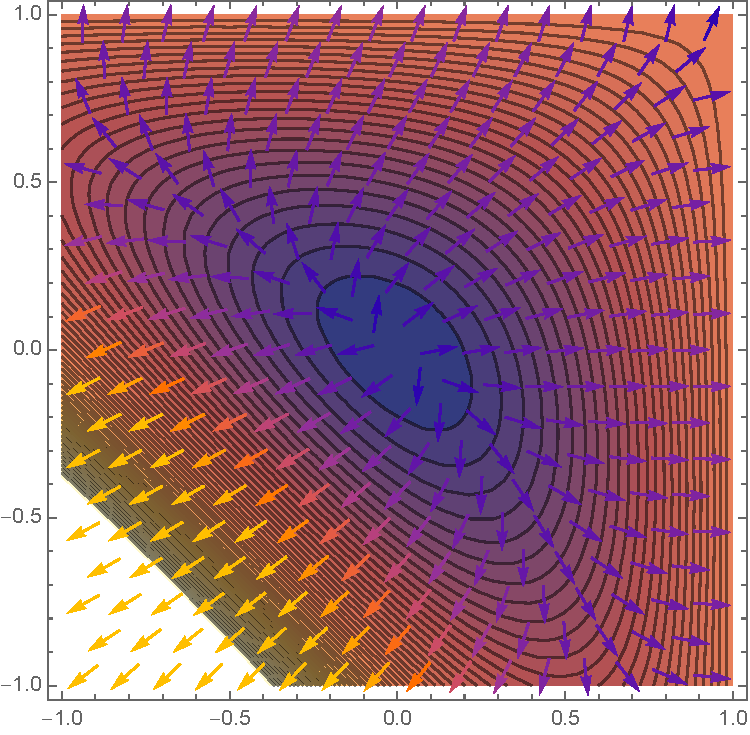
\includegraphics[width=0.49\textwidth]{Ex4ContourF.pdf}}
    \caption{Resultados exerc\'icio 4.}
    \label{fig:grad4}
\end{figure}
\section{Conclusion}\label{sec:conclusion}

% ------- BIBLIOGRAPHY -------
\addcontentsline{toc}{section}{Refer\^encias}
\bibliographystyle{abntex2-num}
\bibliography{References}

% ------- APPENDIX -------
\appendix
\section{GitHub Repository}\label{sec:github}
 The source code for this report and every code inhere mentioned can be found in the following GitHub repository: \href{https://github.com/CarlosPuga14/MetodosNumericos_2024S1}{CarlosPuga14/MetodosNumericos\_2024S1}.

\end{document}